\section{Simple Sampling - Integration}
In this worksheet we will use the Monte Carlo technique to integrate a function and to look at the Ising 
spin model. The Monte Carlo method is a statistical technique for computing expectation values that are 
given by
\begin{equation}
\langle A \rangle = \frac{\int_\Phi A(\phi) P(\phi) d\phi}{\int P(\phi) d\phi}
\label{eq:exp}
\end{equation}
where $A$ is an observable, $P$ is the probability of finding the system in a certain state, $\phi$ is a state of the system and $\Phi$ is the set of all states of the system.

The Monte Carlo simply replaces these integrals with finite sums over random states of the system as
\begin{equation}
\langle A \rangle = \frac{\sum_N A(\phi) P(\phi) d\phi}{\sum_N P(\phi) d\phi}.
\label{eq:mc}
\end{equation}
If the states $\phi$ are randomly distributed then this is called simple sampling.

We can use the Monte Carlo method to evaluate an integral if we set $\phi = x$ and let $P(x)$ be constant. Equate eqs. \ref{eq:exp} and \ref{eq:mc} and solve for the integral leaves us with
\begin{equation}
\int_a^b f(x) dx = \frac{b-a}{N} \sum_N f(x_i)
\label{eq:int}
\end{equation}
where we have renamed $A$ to $f$.

We begin this worksheet by using this method to evaluate the integral of the Runge function over the interval $[-5, 5]$. The Runge function is given by
\begin{equation}
f(x) = \frac{1}{1+x^2}
\end{equation}
and its integral is 
\begin{equation}
\int_a^b \frac{1}{1+x^2} dx = \arctan(b)-\arctan(a).
\end{equation}

We begin by writing a simple function in python to compute the Runge function and another to compute its integral.
\listfile{../src/mon_car.py}{src/mon\_car.py}{3}{7}{Runge Function}{runge}
\begin{figure}[ht]
	\centering
	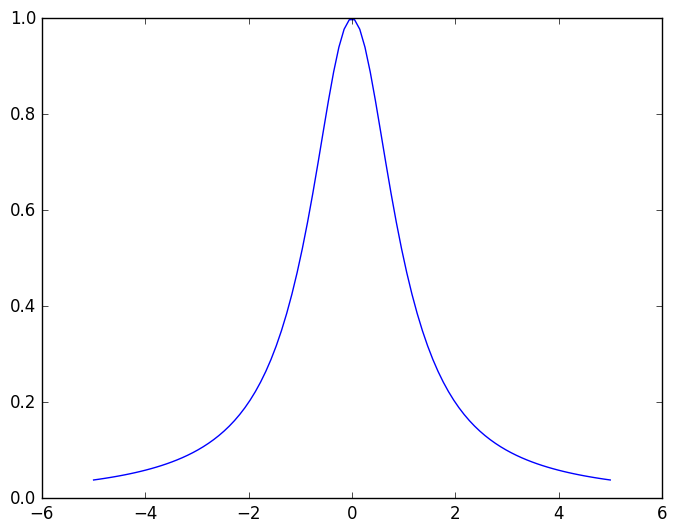
\includegraphics[width=0.7\textwidth]{../fig/rungeplot.png}
	\caption{Plot of the Runge function from $-5$ to $5$.	}
	\label{fig:runge}
\end{figure}
The Runge function is plotted in fig. \ref{fig:runge}

Now we will use a simple sampling Monte Carlo technique to evaluate the integral. Equation \ref{eq:int} is implemented as:
\listfile{../src/mon_car.py}{src/mon\_car.py}{9}{12}{Simple Sampling}{simple}
This allows us to set a function, upper and lower bound, and number of samples as parameters. The measured value of the integral and the standard error of the mean are returned. 

We now write a program to use our Monte Carlo algorithm to compute this integral for a number of samples $N = 2^i$ with $2 \leq i \leq 20$. 
\listfile{../src/integration.py}{src/integration.py}{5}{13}{Simple Sampling}{simpsamp}
\begin{figure}[ht]
	\centering
	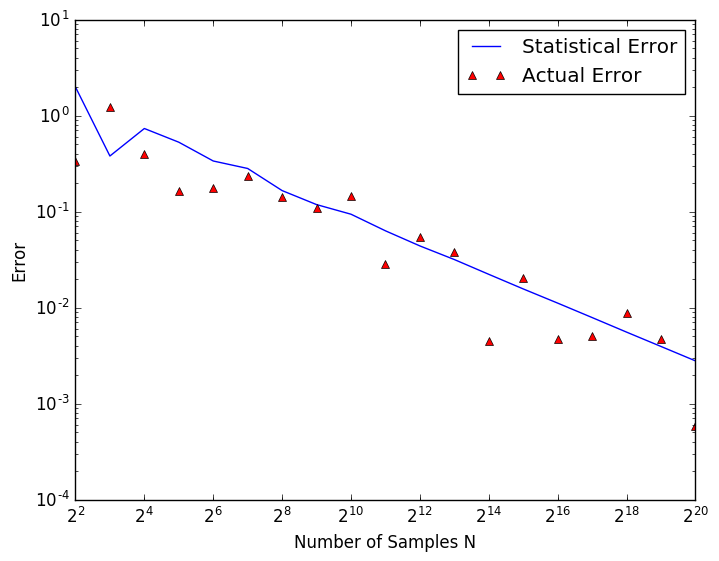
\includegraphics[width=0.7\textwidth]{../fig/simple_err.png}
	\caption{Plot of the statistical vs actual error in our simple sampling evaluation of the integral of the Runge function for various number of samples.	}
	\label{fig:simple}
\end{figure}
Figure \ref{fig:simple} shows the statistical vs. actual error in our calculation of this integral for our range of samples. We used a log-log plot for readability.
